\section{Motivating case study: \texorpdfstring{\gls{lkas}}{lkas}}
\label{sec:lkas_case_Study}
This thesis uses the motivating case study of a \gls{lkas}.
\begin{figure}
\centerline{
    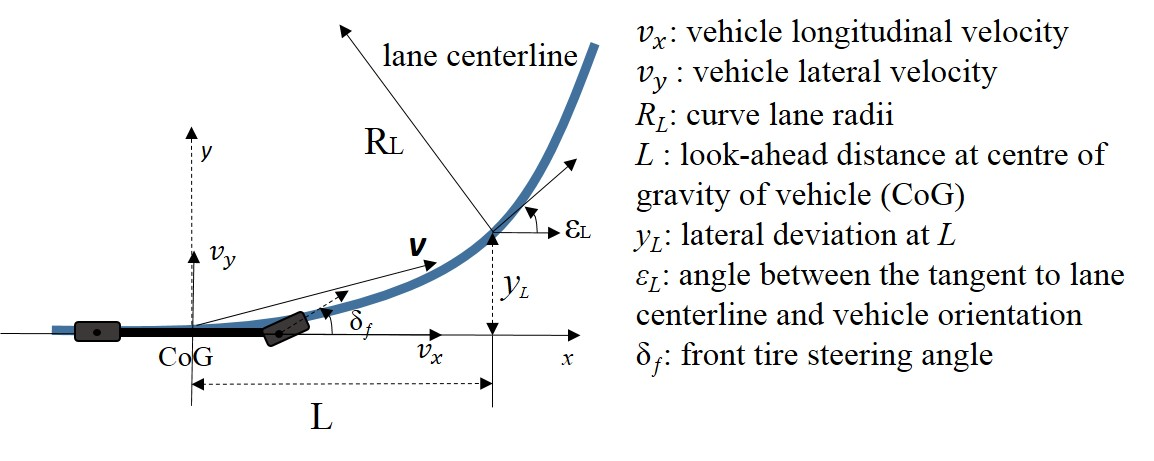
\includegraphics[width=\textwidth]{01_intro/images/model.jpg}
    }
    \vspace{-1em}
    \caption{\Gls{lkas} dynamics model derived from~\cite{kosecka1997vision}.}
    \label{fig:intro_model_lateral_control}
    %\vspace{-1em}
\end{figure}
The bicycle model derived from~\cite{kosecka1997vision} (illustrated in Fig.~\ref{fig:intro_model_lateral_control}) is considered for simulating the \gls{lkas} of a vehicle\footnote{The (default) vehicle parameters are those specified in~\cite{kosecka1997vision} for Honda Accord.} on a straight road and it is described as follows,
\begin{align*}
  \Acont (v_x)&= \left[
  \begin{array}{cccc}
    -\frac{c_{f}+c_{r}}{mv_{x}} & \frac{-mv_{x}^2+c_{r}l_{r}-c_{f}l_{f}}{mv_{x}} & 0  & 0\\
    \frac{-l_{f}c_{f}+l_{r}c_{r}}{I_{\psi}v_{x}} & -\frac{l_{f}^2c_{f}+l_{r}^2c_{r}}{I_{\psi}v_{x}} & 0 & 0\\
    -1 & -L & 0 & v_{x} \\
    0 & -1 & 0 & 0
  \end{array}
\right],\\ \Bcont &=\left[
  \begin{array}{cccc}
    \frac{c_{f}}{m} &
    \frac{l_{f}c_{f}}{I_{\psi}} &
    0&
    0
  \end{array}
\right]^{\top},\\ 
 \Ccont &=\left[
  \begin{array}{cccc}
    0 &
    0 &
    1&
    0
  \end{array}
\right], \\
\Dcont &=\textbf{0},
\end{align*}
 where, referring to Fig.~\ref{fig:intro_model_lateral_control}, we define the state vector $x(t) = [v_{y}, \dot{\psi}, \yL, \varepsilon_{L}]$, the measured output $y(t)$ as $\yL$, and the control input $u(t)$ as the steering angle $\delta_f$, where
$\dot{\psi}$ is the vehicle's yaw rate in rad/s, where the velocity components $v_x$ and $v_y$ are in m/s, where $l_{f}$,\ $l_{r}$ ($=1.22$ and $1.62$ m respectively) denote distance of the front and rear axles from the \gls{cog}, where 
$I_{\psi}$ ($=2920$ kg$\cdot$m$^2$) is the total inertia of the vehicle around its \gls{cog}, where
$c_{f}$,\ $c_{r}$ (${=1.2\times10^5\text{~N/rad)}}$ denote cornering stiffness of the front and rear tires, and where the total mass of the vehicle is $m$ ($=1590$ kg). Note that the model can be either linear time-invariant or time-variant depending on whether longitudinal velocity $v_x$ is constant or time-varying. 